\chapter{State of the Art}
\graphicspath{{state-of-the-art/figures/}}

In recent years, the remarkable advancements in Natural Language Processing (NLP) have been primarily driven by the development of LLMs. These LLMs, such as GPT (Generative Pretrained Transformer) and BERT (Bidirectional Encoder Representations from Transformers), have demonstrated remarkable capabilities in understanding and generating human-like text. However, despite their impressive performance, LLMs still face challenges in effectively retrieving and incorporating relevant context for generating accurate and coherent responses.

Enter RAG systems, a novel approach that seeks to overcome the limitations of traditional LLMs by integrating retrieval mechanisms with generation models. RAG systems combine the strengths of both retrieval and generation techniques to enhance the quality and relevance of generated text.

This chapter provides a comprehensive exploration of RAG systems, delving into their architecture, components, training processes, applications, advantages, and challenges. We begin by establishing a foundational understanding of LLMs and their evolution, laying the groundwork for understanding the need for RAG systems. We then proceed to dissect the intricacies of RAG systems, discussing the role of retrieval in providing context and the role of generation in producing fluent responses.

Through detailed examination and analysis, we uncover the inner workings of RAG systems, exploring how retrieval and generation components interact within the architecture. Real-world applications and use cases of RAG systems across various domains are elucidated, demonstrating their potential to revolutionize tasks such as question answering, dialogue generation, and content creation.

Furthermore, we evaluate the advantages and limitations of RAG systems compared to traditional LLMs and other approaches in NLP. By examining performance metrics, challenges, and future directions, we gain insights into the transformative impact of RAG systems on the field of natural language processing.

In summary, this chapter serves as a comprehensive guide to RAG systems, offering readers a deep dive into one of the most promising advancements in NLP. As we navigate through the complexities and potentials of RAG systems, we pave the way for understanding their role in shaping the future of human-computer interaction and language understanding.

\section{Machine Learning}

\subsection{Definition}

Machine learning (ML) is a field of study in artificial intelligence concerned with the development and study of statistical algorithms that can learn from data and generalize to unseen data, and thus perform tasks without explicit instructions. Recently, artificial neural networks have been able to surpass many previous approaches in performance .

ML finds application in many fields, including natural language processing, computer vision, speech recognition, email filtering, agriculture, and medicine. When applied to business problems, it is known under the name predictive analytics. Although not all machine learning is statistically based, computational statistics is an important source of the field's methods \cite{enwiki:1220758567}.

\subsection{Relationships to other fields}

Artificial Intelligence (AI) encompasses the field of computer science dedicated to creating systems capable of emulating human-like intelligence, problem-solving, and decision-making. Machine Learning (ML) is a subset of AI focused on enabling computers to learn from data without being explicitly programmed. Within ML, Deep Learning stands out as a subfield that employs neural networks with multiple layers to learn complex representations of data, particularly effective in tasks like image and speech recognition. ML and Deep Learning are integral components of AI, providing the framework for developing intelligent systems capable of learning, reasoning, and adapting to new information, thereby advancing the capabilities of AI across various domains.

\begin{figure}[htpb]
    \centering
    \includegraphics[width=\textwidth,height=6cm,keepaspectratio=true]{ml.png}
    \caption{
        Machine learning as subfield of AI, from \cite{enwiki:1220758567}.
    }
\end{figure}

\subsection{Types of Machine Learning}

Machine Learning can be broadly categorized into several types based on the learning approach, the availability of labeled data, and the feedback mechanism. The main types of machine learning are:

\begin{figure}[htpb]
    \centering
    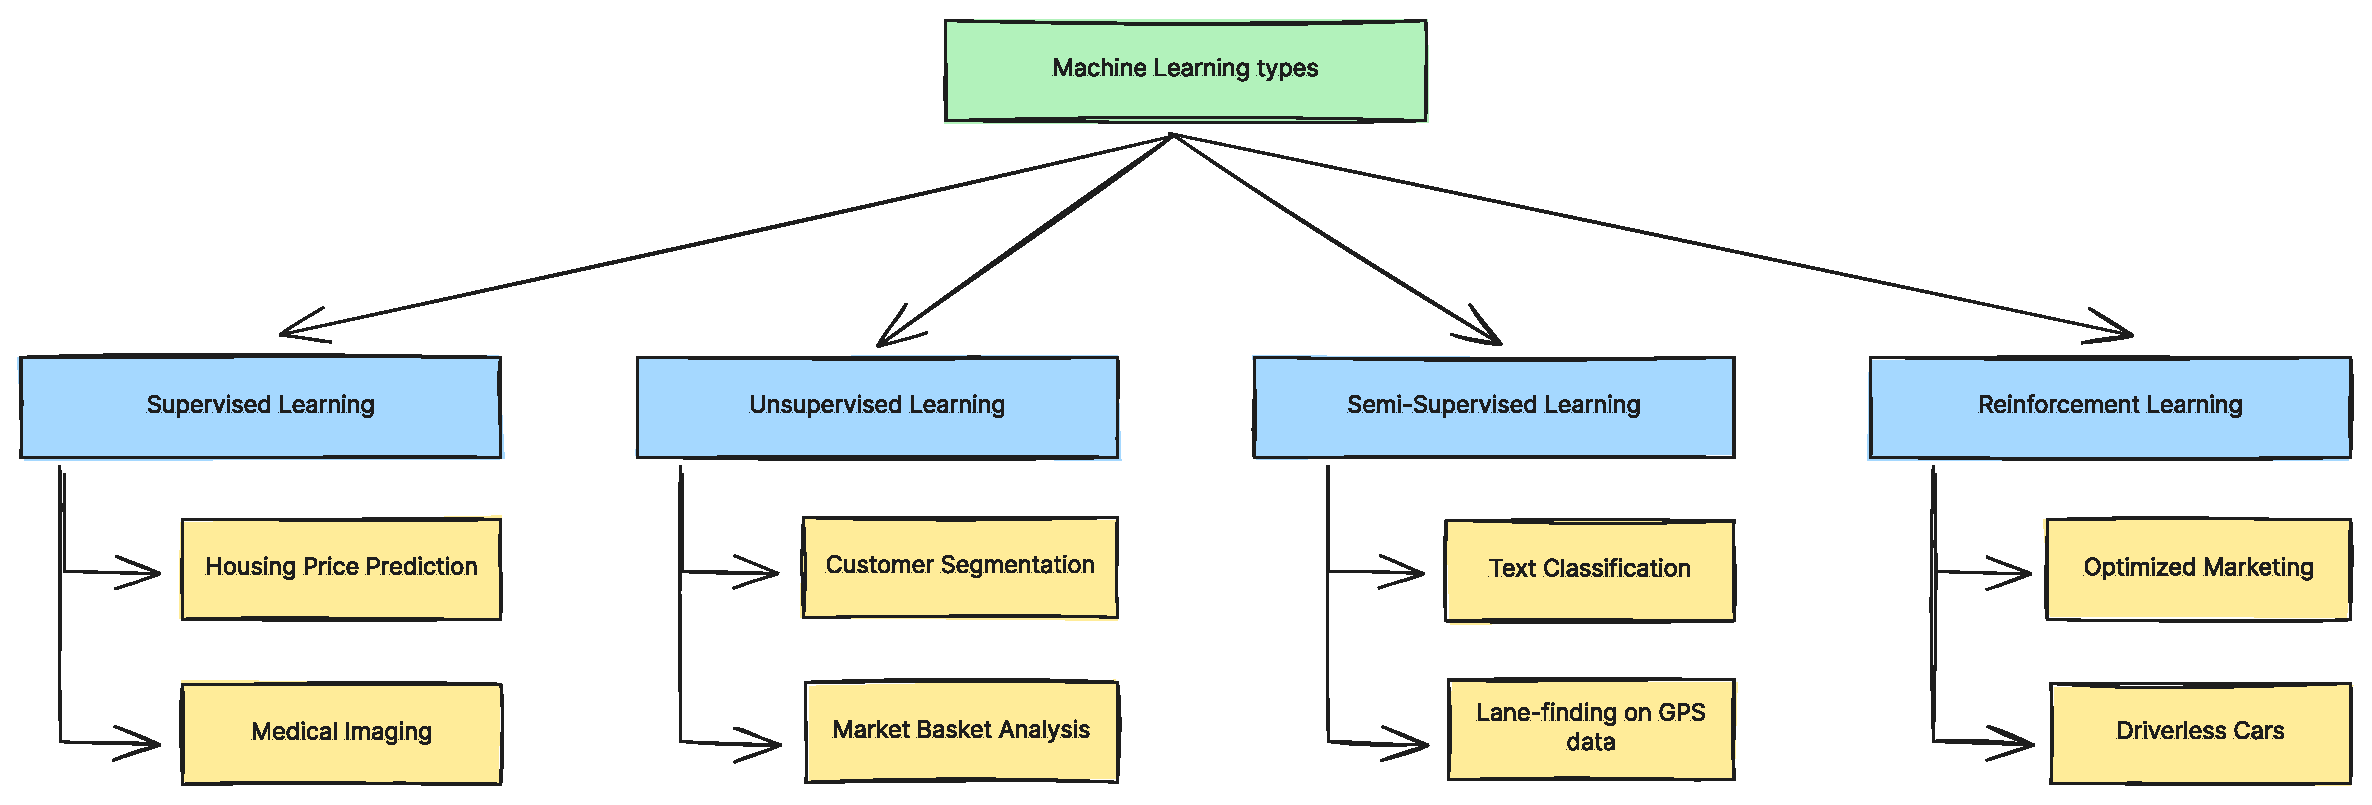
\includegraphics[width=\textwidth,height=6cm,keepaspectratio=true]{ml-types.pdf}
    \caption{
        Types of machine Learning.
    }
\end{figure}

\subsubsection*{Supervised Learning}

\begin{itemize}
    \item{In supervised learning, the algorithm learns from labeled data, where each input example is paired with the corresponding output label.}
    \item{The goal is to learn a mapping from inputs to outputs, allowing the algorithm to make predictions or classifications on unseen data.}
    \item{Common supervised learning tasks include regression (predicting continuous values) and classification (predicting discrete labels).}
\end{itemize}

\subsubsection*{Unsupervised Learning:}

\begin{itemize}
    \item{Unsupervised learning involves learning from unlabeled data, where the algorithm aims to find patterns, structures, or relationships in the data without explicit guidance.}
    \item{The algorithm discovers hidden structures or clusters within the data, facilitating tasks such as clustering, dimensionality reduction, and anomaly detection.}
\end{itemize}

\subsubsection*{Semi-Supervised Learning:}

\begin{itemize}
    \item{Semi-supervised learning lies between supervised and unsupervised learning, where the algorithm learns from a combination of labeled and unlabeled data.}
    \item{The presence of both labeled and unlabeled data allows the algorithm to leverage additional information and improve performance, particularly in scenarios where labeled data is scarce or expensive to obtain.}
\end{itemize}

\subsubsection*{Reinforcement Learning:}

\begin{itemize}
    \item{Reinforcement learning involves an agent learning to make decisions by interacting with an environment to achieve a specific goal.}
    \item{The agent receives feedback in the form of rewards or penalties based on its actions, enabling it to learn through trial and error.}
    \item{Reinforcement learning is commonly used in applications such as game playing, robotics, and autonomous systems.}
\end{itemize}

\subsection{Limitations of Machine Learning: Challenges and Considerations}

Although machine learning is a powerful technique for extracting knowledge from data, it also has certain limitations that are important to consider:

\begin{itemize}
    \item{\textbf{Data dependency:} Machine learning heavily relies on the quality and quantity of training data. If the data is poorly labeled or unrepresentative, it can lead to errors in predictions.}
    \item{\textbf{Overfitting:} When the model is too complex compared to the training data, it can overfit and not generalize well to test data. This can also result in poor performance for new data.}
    \item{\textbf{Explainability:} Machine learning models can be very complex and difficult to understand. It can be challenging to understand how the model makes decisions and to explain these decisions to users.}
    \item{\textbf{Biased data:} Training data can be biased due to factors such as data selection, human biases, or measurement errors. This can lead to biased predictions for test data.}
    \item{\textbf{Lack of diversity:} Machine learning models may lack diversity in the types of data they can handle. For example, machine learning models may struggle to process unstructured data such as images, sounds, and texts.}
    \item{\textbf{Computational cost:} Machine learning algorithms may require high computational power and significant storage resources to process large amounts of data. This can be costly and time-consuming to train and implement models.}
\end{itemize}
